\PassOptionsToPackage{unicode=true}{hyperref} % options for packages loaded elsewhere
\PassOptionsToPackage{hyphens}{url}
%
\documentclass[]{article}
\usepackage{lmodern}
\usepackage{amssymb,amsmath}
\usepackage{ifxetex,ifluatex}
\usepackage{fixltx2e} % provides \textsubscript
\ifnum 0\ifxetex 1\fi\ifluatex 1\fi=0 % if pdftex
  \usepackage[T1]{fontenc}
  \usepackage[utf8]{inputenc}
  \usepackage{textcomp} % provides euro and other symbols
\else % if luatex or xelatex
  \usepackage{unicode-math}
  \defaultfontfeatures{Ligatures=TeX,Scale=MatchLowercase}
\fi
% use upquote if available, for straight quotes in verbatim environments
\IfFileExists{upquote.sty}{\usepackage{upquote}}{}
% use microtype if available
\IfFileExists{microtype.sty}{%
\usepackage[]{microtype}
\UseMicrotypeSet[protrusion]{basicmath} % disable protrusion for tt fonts
}{}
\IfFileExists{parskip.sty}{%
\usepackage{parskip}
}{% else
\setlength{\parindent}{0pt}
\setlength{\parskip}{6pt plus 2pt minus 1pt}
}
\usepackage{hyperref}
\hypersetup{
            pdftitle={Electrophysiological measures of visual suppression},
            pdfauthor={Daniel H. Baker \& Alex R. Wade},
            pdfborder={0 0 0},
            breaklinks=true}
\urlstyle{same}  % don't use monospace font for urls
\usepackage[margin=1in]{geometry}
\usepackage{longtable,booktabs}
% Fix footnotes in tables (requires footnote package)
\IfFileExists{footnote.sty}{\usepackage{footnote}\makesavenoteenv{longtable}}{}
\usepackage{graphicx,grffile}
\makeatletter
\def\maxwidth{\ifdim\Gin@nat@width>\linewidth\linewidth\else\Gin@nat@width\fi}
\def\maxheight{\ifdim\Gin@nat@height>\textheight\textheight\else\Gin@nat@height\fi}
\makeatother
% Scale images if necessary, so that they will not overflow the page
% margins by default, and it is still possible to overwrite the defaults
% using explicit options in \includegraphics[width, height, ...]{}
\setkeys{Gin}{width=\maxwidth,height=\maxheight,keepaspectratio}
\setlength{\emergencystretch}{3em}  % prevent overfull lines
\providecommand{\tightlist}{%
  \setlength{\itemsep}{0pt}\setlength{\parskip}{0pt}}
\setcounter{secnumdepth}{5}
% Redefines (sub)paragraphs to behave more like sections
\ifx\paragraph\undefined\else
\let\oldparagraph\paragraph
\renewcommand{\paragraph}[1]{\oldparagraph{#1}\mbox{}}
\fi
\ifx\subparagraph\undefined\else
\let\oldsubparagraph\subparagraph
\renewcommand{\subparagraph}[1]{\oldsubparagraph{#1}\mbox{}}
\fi

% set default figure placement to htbp
\makeatletter
\def\fps@figure{htbp}
\makeatother


\title{Electrophysiological measures of visual suppression}
\author{Daniel H. Baker \& Alex R. Wade}
\date{2021-02-15}

\begin{document}
\maketitle

\hypertarget{abstract}{%
\section{Abstract}\label{abstract}}

\hypertarget{introduction}{%
\section{Introduction}\label{introduction}}

Suppression is a fundamental component of the nervous system, and is critically important for moderating neural firing. Without suppression, neural activity would be too metabolically expensive, and uncontrolled excitation would lead to seizures. In the visual system, neurons responsive to a spatially localised stimulus of a given orientation are suppressed by nearby neurons that differ in their tuning. This tuning might involve different orientations (cross-orientation suppression), different spatial locations (lateral, or surround suppression), and different eye-of-origin (interocular suppression).

Several studies have demonstrated that these different types of suppression occur at different stages in the early visual pathway, and therefore have different characteristics. Baker et al. (2007) Petrov et al. (2005) Li et al. (2005)

In addition, there is evidence that suppression builds up at successive stages of cortical processing, beyond primary visual cortex, and is stronger at later levels in the visual hierarchy.

An important distinction concerns whether a suppressive effect modulates the contrast gain or the response gain of a neuron. Changes in contrast gain shift the stimulus-response curve (the contrast response function) laterally, whereas changes in response gain scale the function vertically (see examples in Figure \ref{fig:stimfig}c). These different patterns may be indicative of specific neurophysiological underpinnings for an effect. Additionally, both processes might occur at successive stages of processing.

\begin{figure}

{\centering 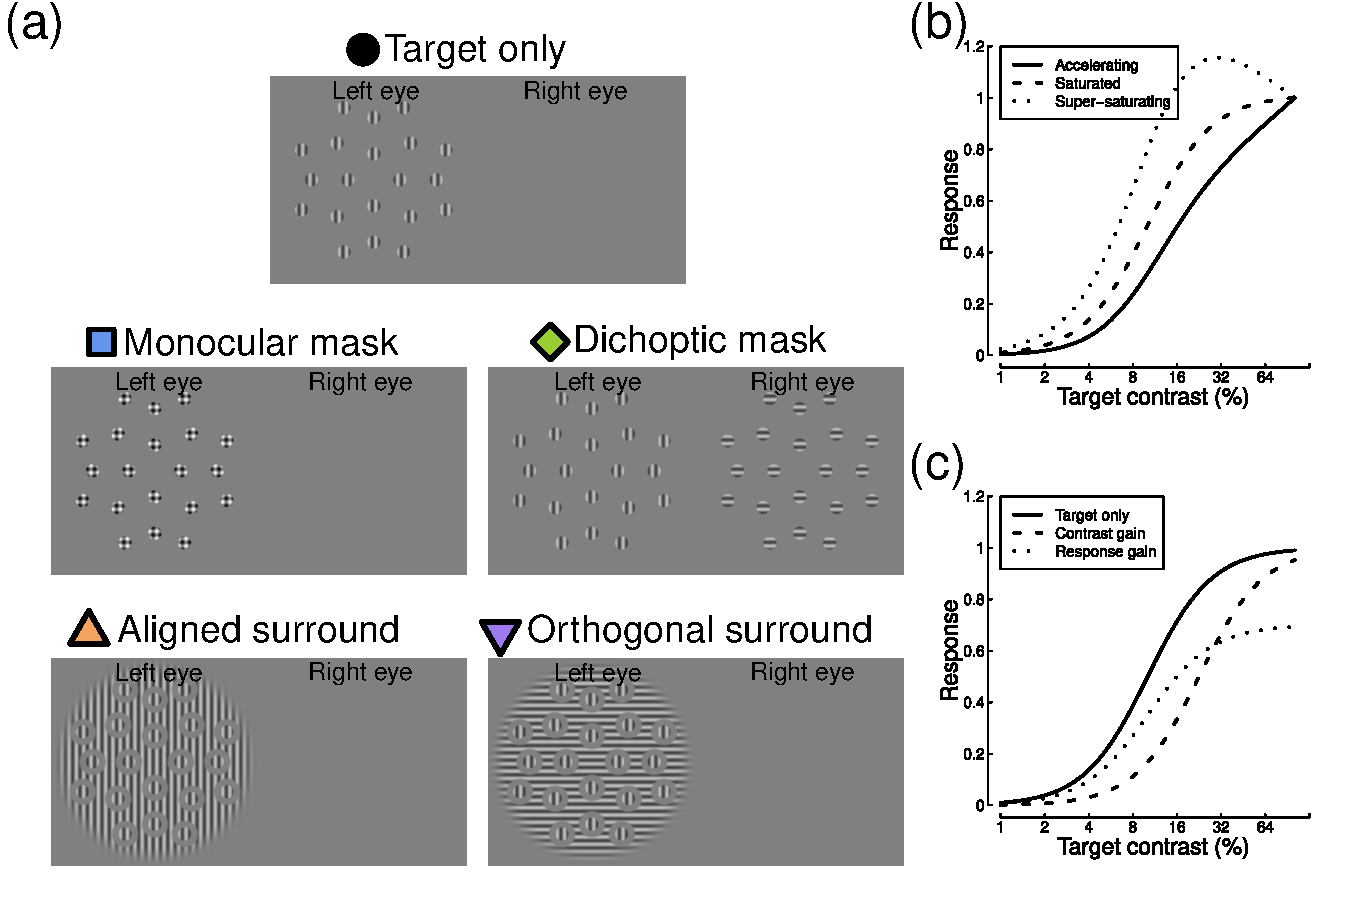
\includegraphics{figures/stimfig} 

}

\caption{Example stimuli and illustration of contrast response functions.}\label{fig:stimfig}
\end{figure}

In this study, we measured four types of suppression in human participants using a steady-state evoked potential (SSVEP) technique. Target stimuli flickered at a known frequency (5Hz), and frequency-locked responses were measured using electroencephalography (EEG). Note that the SSVEP technique records ensemble activity of populations of neurons that are responsive to the target stimulus. Our primary motivation was to compare the suppressive effects from different mask types (monocular, dichoptic, and two types of surround mask), to determine whether they are best described as contrast or response gain modulation, and to explore how suppression changes at successive stages of processing. We repeated the experiment at two different mask contrasts, and analyse the data using a Bayesian modelling approach.

\hypertarget{methods}{%
\section{Methods}\label{methods}}

\hypertarget{participants}{%
\subsection{Participants}\label{participants}}

Twelve participants completed each version of the experiment (3 participants completed both experiments, the remaining 9 were unique to each experiment). All participants had normal or corrected-to-normal vision, and no known visual abnormalities. All participants provided written informed consent.

\hypertarget{apparatus-and-stimuli}{%
\subsection{Apparatus and stimuli}\label{apparatus-and-stimuli}}

Stimuli were presented using a ViewPixx 3D display, driven by a Mac Pro computer. The display updated at 120 Hz, and we interleaved frames intended for the left and right eyes (60 Hz refresh rate per eye). The display update was synchronised with a set of NVidia 3D pro active shutter glasses using an infra-red signal. The display had a resolution of 1920 \(\times\) 1280 pixels, and was viewed from a distance of 57cm, at which one degree of visual angle had a diameter of 36 pixels. The display was run in the high bit-depth monochrome M16 mode, which provided 16 bits of greyscale resolution. The display was gamma corrected using a Minolta LS110 photometer and had a maximum luminance of 102 \(cd/m^2\).

All stimuli were patches of sinusoidal grating with a spatial frequency of 1 cycle per degree. Target stimuli were randomly oriented on each trial, and windowed by a raised cosine envelope with a width of 2 degrees. There were 20 targets arranged in a symmetrical pattern around a central fixation marker, as shown in Figure \ref{fig:stimfig}. The target eccentricities were 3.6, 7.1, 8.5 and 10.7 degrees from the central fixation. Stimuli were placed at 90 degree intervals at each radius, or in 45 degree intervals at the largest eccentricity. All target stimuli flickered sinusoidally at 5Hz (on-off flicker), between 0\% contrast and their nominal Michelson contrast, which was one of six values (0, 6, 12, 24, 48 and 96\%). Percentage Michelson contrast is defined as \(100\frac{L_{max}-L_{min}}{L_{max}+L_{min}}\), where \emph{L} is luminance. Targets were shown to one eye only, which was chosen randomly on each trial. A binocular fixation marker was created from a cluster of overlaid squares (each 13 arc min wide) with random grey levels, designed to aid binocular fusion. Similar markers were also presented in the four corners of the stimulus region, at a distance of 15.7 degrees from the display centre.

We measured target responses with no mask, and also with four categories of mask stimulus. Monocular masks were shown to the same eye as the targets and in the same locations, but had orthogonal orientation. Dichoptic masks were the same, but shown to the non-target eye. Aligned surround masks were large (28 degrees) grating patches with the same orientation as the target, and with holes surrounding each target element (and the fixation marker). The holes were 4 degrees in diameter, meaning the gap between target and mask was 1 degree. Orthogonal surrounds were the same, but were oriented at 90 degrees relative to the targets. There were two principal mask contrasts that were used in the two versions of the experiment: 12\% and 24\%. We also tested several additional mask contrasts (6, 48 and 96\% contrast) for a single target contrast of 24\%. The masks drifted at a speed of 6 deg/sec so that the phase alignment between mask and target changed over time. Note that drifting gratings do not produce a steady-state signal, so we did not record responses to the mask stimuli. Also, for some of the monocular mask conditions, the stimulus contrast was reduced from 96\% to 68\% to avoid clipping artifacts caused by overlaying the target and mask.

EEG activity was recorded using a 64-channel ANT Neuroscan system sampling at 1 kHz. Participants wore Waveguard caps, with electrodes organised according to the 10/20 system. The ground was located at position \emph{AFz}, and each channel was referenced to the whole-head average. Electrode impedance was maintained at or below \(5k\Omega\) throughout the experiment. Digital parallel triggers were sent from the ViewPixx display to the EEG amplifier, and recorded the onset of each trial on the EEG trace. Data were amplified, digitised, and saved to disc for offline analysis.

\hypertarget{procedure}{%
\subsection{Procedure}\label{procedure}}

\hypertarget{data-analysis-and-modelling}{%
\subsection{Data analysis and modelling}\label{data-analysis-and-modelling}}

\hypertarget{data-and-script-availability}{%
\subsection{Data and script availability}\label{data-and-script-availability}}

All data and scripts are publicly available at:

\hypertarget{results}{%
\section{Results}\label{results}}

\hypertarget{discussion}{%
\section{Discussion}\label{discussion}}

\hypertarget{acknowledgements}{%
\section{Acknowledgements}\label{acknowledgements}}

Supported by the Royal Society (grant number RG130121 to DHB).

\hypertarget{references}{%
\section*{References}\label{references}}
\addcontentsline{toc}{section}{References}

\hypertarget{refs}{}
\leavevmode\hypertarget{ref-Baker2007}{}%
Baker DH, Meese TS, Summers RJ. 2007. Psychophysical evidence for two routes to suppression before binocular summation of signals in human vision. \emph{Neuroscience} \textbf{146}:435--48. doi:\href{https://doi.org/10.1016/j.neuroscience.2007.01.030}{10.1016/j.neuroscience.2007.01.030}

\leavevmode\hypertarget{ref-Li2005}{}%
Li B, Peterson MR, Thompson JK, Duong T, Freeman RD. 2005. Cross-orientation suppression: Monoptic and dichoptic mechanisms are different. \emph{J Neurophysiol} \textbf{94}:1645--50. doi:\href{https://doi.org/10.1152/jn.00203.2005}{10.1152/jn.00203.2005}

\leavevmode\hypertarget{ref-Petrov2005}{}%
Petrov Y, Carandini M, McKee S. 2005. Two distinct mechanisms of suppression in human vision. \emph{J Neurosci} \textbf{25}:8704--7. doi:\href{https://doi.org/10.1523/JNEUROSCI.2871-05.2005}{10.1523/JNEUROSCI.2871-05.2005}

\end{document}
